% Provenance (never printed): see sources/outline_sources.md (Year 1:
% observational astronomy, photometry). Telescopes, angular resolution,
% gratings, the Doppler effect and the black-body laws are owned by the
% physics series and recalled here. Curves computed in
% figdata/bachelor-1/{blackbody_bands, extinction_line}.py; numbers of the
% exercises and problem in the Book 3 scratch calculator ch02.py.
\chapter{Telescopes, Detectors and Photometry}\label{ch:b1:observing-the-sky}

Everything astronomy knows about the stars, apart from a few meteorites and
the samples brought back from the Moon and from asteroids, it has learnt from
the light they send. That light crosses the Earth's atmosphere, which absorbs
whole ranges of wavelength and blurs the rest; it is gathered by a mirror
whose size limits both how faint and how fine the details can be; it is
counted by a detector that turns photons into electrons, and every count
carries a statistical uncertainty. Before a brightness becomes a \omterm{def:b1:observing-the-sky:flux}{luminosity}
or a distance, each of these steps has to be understood and corrected. This
chapter follows the light from the star to the number: the windows of the
atmosphere and the extinction law, the telescope and the \omterm{def:b1:observing-the-sky:seeing}{seeing}, the
detector and its noise, then the magnitudes, parallaxes and colours that
turn measured \omterm{def:b1:observing-the-sky:flux}{fluxes} into the properties of stars. The same atmosphere, seen
from below, is the subject of the climate chapters
(\cref{ch:b1:radiation-heat-transport}); the same photometry, applied to
planets, opens the next chapter (\cref{ch:b1:comparative-planetology}).

\begin{recall}
A telescope's objective collects light over its aperture and forms an image
at its focus; diffraction by an aperture of diameter $D$ limits the smallest
angle it separates to about $1.22\,\lambda/D$, the Rayleigh criterion (the
physics books' Year 1 volume). A grating disperses light by wavelength
(Year 2), and a source moving along the line of sight shifts its spectral
lines by the Doppler effect (grade 12). A body in thermal equilibrium emits
the black-body spectrum, whose peak obeys Wien's law (Year 2). In chemistry,
the absorbance of a solution grows in proportion to the path length.
\end{recall}

\section{The atmosphere's windows}

The atmosphere is transparent to some wavelengths and opaque to others.
Radiation is absorbed mainly by water vapour, carbon dioxide and ozone, and
at the shortest wavelengths by the atoms and molecules of the upper
atmosphere themselves.
% ledger: nasa:ems-absorbers

\begin{definition}[Atmospheric window]\label{def:b1:observing-the-sky:window}
An \emph{atmospheric window}\index{atmospheric window} is a range of
wavelengths in which the atmosphere transmits most of the radiation that
reaches its top down to the ground. The \emph{optical window} extends from
the near ultraviolet to the near infrared; the \emph{radio window} from
wavelengths of about a centimetre to about ten metres.
\end{definition}

The figure below sketches the opacity of the
atmosphere from gamma rays to long radio waves. Gamma rays, X-rays and
ultraviolet below about \qty{0.3}{\micro\metre} never reach the ground:
they are observed from space. Visible light passes, with some blurring. Most
of the infrared is absorbed by water vapour and carbon dioxide, except in
narrow windows that ground observatories at high, dry sites exploit; the
near-infrared \omterm{def:b1:observing-the-sky:magnitude}{photometric bands} sit in them, at \qty{1.24}{\micro\metre},
\qty{1.65}{\micro\metre} and \qty{2.16}{\micro\metre}. Wavelengths from about
\qty{30}{\micro\metre} to a millimetre are blocked again; radio waves of a
few centimetres to about ten metres pass, even through clouds; longer ones
are reflected by the ionosphere.
% ledger: nasa:opacity-windows, baldry:2mass-pivot

\begin{omfigure}
\begin{tikzpicture}[x=1.0cm, y=2.2cm, font=\scriptsize]
% x = log10(lambda / 1 m) + 10 ; opacity 0..1 (schematic, after the NASA figure)
\fill[omSea!20] (0,0) rectangle (13,1.05);
\fill[brown!50] (0,0) -- (0,1) -- (3.45,1) -- (3.52,0.05) -- (4.03,0.05)
  -- (4.06,0.6) -- (4.09,0.15) -- (4.15,0.6) -- (4.22,0.15) -- (4.28,0.6)
  -- (4.34,0.15) -- (4.42,0.7) -- (4.55,0.25) -- (4.65,0.8) -- (4.9,0.2)
  -- (5.12,0.2) -- (5.25,0.7) -- (5.4,1) -- (7.0,1) -- (7.3,0.6) -- (7.6,0.75)
  -- (8.0,0.5) -- (8.5,0.03) -- (11.0,0.03) -- (11.3,1) -- (13,1) -- (13,0)
  -- cycle;
\draw[black!70] (0,0) rectangle (13,1.05);
\foreach \x in {0,...,13} { \draw (\x,0) -- (\x,-0.05); }
\foreach \x/\l in {0/0.1 nm, 2/10 nm, 4/1 \textmu m, 6/100 \textmu m, 8/1 cm,
  10/1 m, 12/100 m}
  { \node[below] at (\x,-0.05) {\l}; }
\foreach \y/\l in {0/0, 0.5/50, 1/100}
  { \draw (0,\y) -- (-0.1,\y); \node[left] at (-0.1,\y) {\l}; }
\node[rotate=90] at (-0.75,0.5) {opacity (\%)};
\node at (6.5,-0.42) {\small wavelength (logarithmic scale)};
\node[align=center] at (1.7,0.75) {gamma rays, X-rays,\\ ultraviolet};
\node[align=center] at (6.2,0.75) {far\\ infrared};
\node[align=center] at (9.75,0.5) {radio window};
\node[omThm] at (4.15,0.86) {J H K};
\draw[-{Stealth}] (2.6,1.25) node[above] {optical window} -- (3.75,1.07);
\draw[-{Stealth}] (5.9,1.25) node[above] {infrared windows} -- (4.6,1.07);
\end{tikzpicture}

{\small The opacity of the atmosphere to radiation arriving from space,
from \qty{0.1}{nm} to \qty{1}{km} (logarithmic scale). Schematic, after a
public-domain NASA figure: only the windows matter here, not the exact shape
of each absorption band. J, H and K mark the near-infrared \omterm{def:b1:observing-the-sky:magnitude}{photometric bands}.}
% ledger: nasa:opacity-windows, nasa:ems-absorbers, baldry:2mass-pivot
\end{omfigure}

\subsection*{Extinction}

Even inside the optical window the atmosphere removes part of the light,
by absorption and by scattering off molecules and aerosols. A thin layer of
thickness $\mathrm ds$ along the ray removes a fraction of the intensity
proportional to $\mathrm ds$: $\mathrm dI = -\kappa I\,\mathrm ds$, where
the extinction coefficient $\kappa$ (per metre) depends on the
wavelength and on the composition of the air at that height. This is the
law of the absorbance of a solution, applied to a column of air.

\begin{proposition}[Bouguer's law]\label{prop:b1:observing-the-sky:bouguer}
Along a ray through an absorbing medium, the intensity decreases as
\[
  I = I_0\,e^{-\tau}, \qquad \tau = \int_0^s \kappa\,\mathrm ds' ,
\]
where $I_0$ is the intensity entering the medium and $\tau$, the optical
depth of the path, is a pure number.
For a plane-parallel atmosphere, a star at the \omterm{def:b1:spherical-astronomy:celestial-sphere}{zenith} distance $z$ (the
angle between its direction and the vertical) is seen through the optical
depth $\tau(z) = \tau_0\sec z$, where $\tau_0$ is the optical depth at the
\omterm{def:b1:spherical-astronomy:celestial-sphere}{zenith}.
\end{proposition}

\begin{proof}
The equation $\mathrm dI/I = -\kappa\,\mathrm ds$ separates: integrating from
the top of the atmosphere ($I = I_0$, $s = 0$) to the observer gives
$\ln(I/I_0) = -\int_0^s\kappa\,\mathrm ds'$. In a plane-parallel atmosphere
$\kappa$ depends on the height $y$ alone, and a ray inclined at $z$ to the
vertical travels $\mathrm ds = \mathrm dy/\cos z$ to climb $\mathrm dy$. Hence
$\tau(z) = \int \kappa(y)\,\mathrm dy/\cos z = \tau_0\sec z$.
\end{proof}

\begin{definition}[Airmass, atmospheric extinction coefficient]\label{def:b1:observing-the-sky:extinction}
The \emph{airmass}\index{airmass} $X$ of an observation is the optical depth
of the line of sight divided by the optical depth at the \omterm{def:b1:spherical-astronomy:celestial-sphere}{zenith}:
$X = \tau(z)/\tau_0$. It equals 1 at the \omterm{def:b1:spherical-astronomy:celestial-sphere}{zenith} and, for a plane-parallel
atmosphere, $X = \sec z$. The \emph{atmospheric extinction
coefficient}\index{atmospheric extinction coefficient} $k$ in a given band
is the dimming, in magnitudes, produced by one airmass, so that a star of
magnitude $m_0$ above the atmosphere is observed at
\[
  m = m_0 + kX .
\]
\end{definition}

Magnitudes are defined in \cref{sec:b1:observing-the-sky:magnitudes}; all
that is needed here is that a dimming by the factor $e^{-\tau}$ adds
$2.5\log_{10}e\;\tau = 1.086\,\tau$ magnitudes, so that $k = 1.086\,\tau_0$.
The plane-parallel \omterm{def:b1:observing-the-sky:extinction}{airmass} is excellent down to an \omterm{def:b1:spherical-astronomy:horizontal}{altitude} of about
\ang{30} ($X = 2$) and fails near the horizon, where $\sec z$ grows without
limit while the true path through a curved atmosphere stays finite;
observers avoid low \omterm{def:b1:spherical-astronomy:horizontal}{altitudes} for that reason and for the blurring that
grows with the path.

\begin{method}[The extinction line]\label{met:b1:observing-the-sky:extinction-line}
To find the magnitude $m_0$ that a star would have above the atmosphere:
\begin{enumerate}
  \item measure the magnitude $m$ of the star, or of a standard star, at
        several airmasses through the night, as it rises or sets;
  \item compute each \omterm{def:b1:observing-the-sky:extinction}{airmass} from the \omterm{def:b1:spherical-astronomy:celestial-sphere}{zenith} distance, $X = \sec z$;
  \item plot $m$ against $X$ and fit a straight line by least squares;
  \item the slope is the extinction coefficient $k$ of the night in that
        band; the intercept at $X = 0$ is $m_0$.
\end{enumerate}
The same $k$ then corrects every other star observed that night in the same
band: $m_0 = m - kX$.
\end{method}

\begin{example}
One night, a star was measured six times in the V band:
\begin{center}
\small
\begin{tabular}{lcccccc}
\hline
$X$ & 1.05 & 1.18 & 1.36 & 1.62 & 1.95 & 2.31 \\
$m$ & 8.024 & 8.031 & 8.072 & 8.104 & 8.171 & 8.216 \\
\hline
\end{tabular}
\end{center}
The least-squares line, drawn in the figure below, has
slope $k = \qty{0.160}{\mag}$ per \omterm{def:b1:observing-the-sky:extinction}{airmass} and intercept $m_0 = 7.851$. The
points scatter about it by \num{0.006} magnitudes, the precision of a good
night's photometry. At the \omterm{def:b1:spherical-astronomy:celestial-sphere}{zenith} the star is dimmed by \num{0.16}
magnitudes, a loss of $1 - 10^{-0.4\times0.160} = \qty{14}{\percent}$ of its
light.
\end{example}

\begin{omfigure}
\begin{tikzpicture}
\begin{axis}[omrecord, width=0.62\linewidth, height=5.4cm, xmin=0, xmax=2.5,
  ymin=7.80, ymax=8.28, y dir=reverse, xlabel={airmass $X$},
  ylabel={magnitude $m$}, yticklabel style={/pgf/number format/fixed,
  /pgf/number format/precision=2}, tick label style={font=\scriptsize},
  label style={font=\small}]
\addplot[omThm, line width=0.9pt, dashed] table[x=X, y=m] {figdata/out/bachelor-1-extinction_line-fit.dat};
\addplot[only marks, mark=*, mark size=1.6pt, omDef] table[x=X, y=m] {figdata/out/bachelor-1-extinction_line-obs.dat};
\node[font=\scriptsize, right, fill=white, inner sep=1pt] at (axis cs:0.05,7.83) {$m_0 = 7.851$};
\node[font=\scriptsize, fill=white, inner sep=1pt, rotate=-10] at (axis cs:0.95,8.10) {slope $k = 0.160$};
\end{axis}
\end{tikzpicture}

{\small An extinction line: the magnitude of one star at six airmasses
(dots) and the least-squares line, extrapolated to $X = 0$, the magnitude
above the atmosphere. Magnitudes increase downward: a fainter star sits
lower.}
\end{omfigure}

\subsection*{Seeing}

The air above a telescope is never still. Cells of air of slightly different
temperatures, and therefore of slightly different refractive indices, drift
across the beam and bend it by small random angles, changing many times a
second. The eye sees a star twinkle; a long exposure records a blurred spot
much larger than the diffraction pattern of the telescope.

\begin{definition}[Seeing]\label{def:b1:observing-the-sky:seeing}
The \emph{seeing}\index{seeing} at a site is the angular diameter of the
image of a point source blurred by atmospheric turbulence in a long
exposure, measured as the full width at half maximum of the image, in
seconds of arc.
\end{definition}

The \omterm{def:b1:observing-the-sky:seeing}{seeing} changes from night to night and from hour to hour. Sites are
chosen for it: on the summit of Maunakea, at \qty{4204}{m}, the median
\omterm{def:b1:observing-the-sky:seeing}{seeing} of the free atmosphere is about \ang{;;0.40}, from about \ang{;;0.45}
in winter to \ang{;;0.35} in summer, with the best tenth of the nights below
about \ang{;;0.25}; the same site has a median of only \qty{0.9}{mm} of
precipitable water vapour above it, which opens its infrared windows.
% ledger: cfht:site, cfht:seeing

\section{Telescopes and resolution}

A telescope does two things: it collects light over the area of its
objective, and it forms an image in which details are separated. The
collecting area grows as $D^2$: a mirror twice as wide gathers four times as
many photons in the same time and reaches stars four times fainter. The
resolution is limited by diffraction to about $1.22\,\lambda/D$, and by the
\omterm{def:b1:observing-the-sky:seeing}{seeing}.

\begin{example}
The Canada--France--Hawaii Telescope on Maunakea has an aperture of
\qty{3.58}{m}. At \qty{550}{nm} its diffraction limit is
\[
  1.22\times\frac{\qty{550e-9}{m}}{\qty{3.58}{m}} = \qty{1.87e-7}{rad}
  = \ang{;;0.039},
\]
ten times finer than the median \omterm{def:b1:observing-the-sky:seeing}{seeing} of \ang{;;0.40} at the same site. The
two limits are equal for a mirror of diameter $D = 1.22\lambda/\theta =
1.22\times\qty{550e-9}{m}/(\num{0.40}/\num{206265}) = \qty{0.35}{m}$: any
ground telescope wider than about \qty{35}{cm} is limited by the \omterm{def:b1:observing-the-sky:seeing}{seeing}, not
by its own optics, at visible wavelengths.
% ledger: cfht:aperture, cfht:seeing
\end{example}

A large ground telescope therefore gains collecting area, not sharpness,
unless it corrects the turbulence. \emph{Adaptive optics} does that: a
sensor measures, many times a second, how the wavefront from a bright
star (or from an artificial star made by a laser in the upper atmosphere)
is distorted, and a thin mirror bent by many small actuators cancels the
distortion. The correction works best in the
infrared, where the turbulence is slower and weaker, and over a small field
round the guide star. In space there is no \omterm{def:b1:observing-the-sky:seeing}{seeing} at all.

\section{Detectors}

The eye integrates light for a fraction of a second and responds to a small
fraction of the photons that enter it. Photographic plates integrated for
hours but recorded only a small fraction of the light. Modern astronomy uses
photon detectors made of semiconductors, in which each absorbed photon of
enough energy frees an electron.

\begin{definition}[Quantum efficiency, signal-to-noise ratio]\label{def:b1:observing-the-sky:detector}
The \emph{quantum efficiency}\index{quantum efficiency} $\eta$ of a detector
at a given wavelength is the fraction of the incident photons that it
records, as photoelectrons: $\eta = N_\mathrm{e}/N_\gamma$. The
\emph{signal-to-noise ratio}\index{signal-to-noise ratio} of a measurement
is the measured signal divided by its standard deviation, the typical size
of its random error.
\end{definition}

The \emph{charge-coupled device} (CCD) is the standard detector of the
optical window. It is a thin slab of silicon divided into a grid of pixels,
each a potential well that stores the electrons freed by the photons
absorbed in it during the exposure. At the end of the exposure, voltages
applied in sequence to the electrodes shift the charges from pixel to pixel,
row by row, to a single amplifier that measures them one by one; the image
is the table of the counts. A CCD records a large fraction of the incident
photons over most of the visible, its response is proportional to the light
received up to a maximum charge per pixel (its \emph{full well}), and it can
integrate for hours. Infrared arrays work on the same principle with other
semiconductors, read pixel by pixel.

Photons arrive at random. If a source sends on average $N$ photoelectrons
during an exposure, the count actually recorded fluctuates from one exposure
to the next with the standard deviation $\sqrt N$ (Poisson statistics,
admitted from probability: the counts of rare independent events).

\begin{proposition}[Photon noise]\label{prop:b1:observing-the-sky:snr}
When photon noise from the source alone dominates, a source giving $R$
photoelectrons per second is measured in a time $t$ with the
\omterm{def:b1:observing-the-sky:detector}{signal-to-noise ratio}
\[
  \mathrm{SNR} = \frac{Rt}{\sqrt{Rt}} = \sqrt{Rt} ;
\]
it grows as the square root of the exposure time, and as the diameter of
the telescope (since $R \propto D^2$). The error on the magnitude is then
$\sigma_m \approx 1.086/\mathrm{SNR}$.
\end{proposition}

\begin{proof}
The signal is $N = Rt$ and its standard deviation $\sqrt N$. For the
magnitude, $m = -2.5\log_{10}N + \text{const}$, so a small error $\sigma_N$
gives $\sigma_m = 2.5\log_{10}e\;\sigma_N/N = 1.086/\mathrm{SNR}$.
\end{proof}

To measure a magnitude to \num{0.01} takes an SNR of about 109, that is
about \num{12000} photoelectrons. For faint sources two other terms enter.
The sky itself glows, and every pixel of the star's image collects sky
photons as well, at a rate $B$; and the amplifier adds a read noise $\sigma_r$
to each pixel read. The full expression,
\[
  \mathrm{SNR} = \frac{Rt}{\sqrt{Rt + Bt + n\sigma_r^2}}
\]
over the $n$ pixels of the image, reduces to $\sqrt{Rt}$ for a bright star
and to $R\sqrt t/\sqrt B$ for a source fainter than the sky. Since $B$ grows
with the area of the \omterm{def:b1:observing-the-sky:seeing}{seeing} disc, good \omterm{def:b1:observing-the-sky:seeing}{seeing} pays twice: a sharper image
both separates more and collects less sky (\cref{exo:b1:observing-the-sky:11}).

\begin{inthefield}[A night at the telescope]
Photometry is done with calibrations as much as with stars. Before the night
an observer at a professional observatory takes \emph{bias} frames
(exposures of zero length, which record the electronic offset of each pixel)
and \emph{flat fields} (images of the evenly lit inside of the dome or of the
twilight sky, which map how the sensitivity varies from pixel to pixel and
across the field); the science images are corrected by subtracting the bias
and dividing by the flat. Through the night, standard stars of known
magnitudes are observed at several airmasses to fix the extinction line and
the zero point that converts counts into magnitudes. A night is called
\emph{photometric} when the extinction stays steady enough for this
correction to hold; on the summit of Maunakea, \qty{55}{\percent} of
the nights are photometric.
% ledger: cfht:nights
\begin{center}
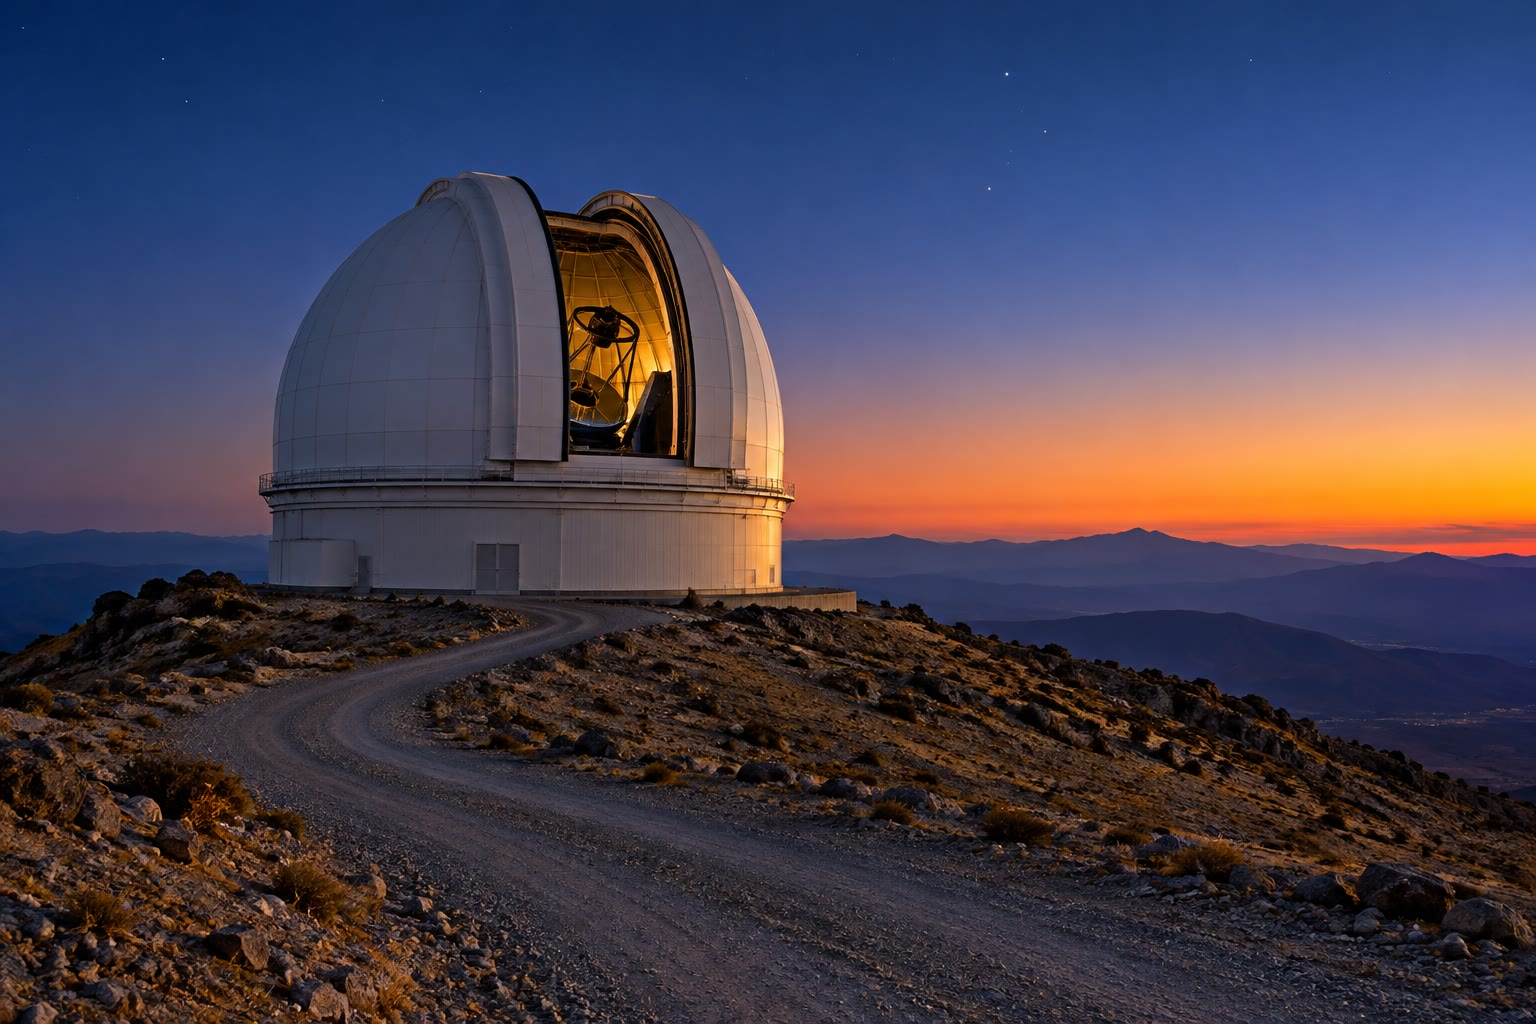
\includegraphics[width=0.55\linewidth]{images/book3/ai/b1-observatory-dusk.jpg}
\end{center}
\end{inthefield}

\section{Fluxes and magnitudes}\label{sec:b1:observing-the-sky:magnitudes}

\begin{definition}[Flux, luminosity]\label{def:b1:observing-the-sky:flux}
The \emph{flux}\index{flux (of a source)} $F$ received from a source is the
power of its radiation crossing a unit area held perpendicular to its
direction, in watts per square metre; restricted to a band of wavelengths,
it is the flux in that band. The \emph{luminosity}\index{luminosity} $L$ of
the source is the total power it radiates, in watts.
\end{definition}

\begin{proposition}[Inverse-square law]\label{prop:b1:observing-the-sky:inverse-square}
A source of \omterm{def:b1:observing-the-sky:flux}{luminosity} $L$ radiating equally in all directions, seen at a
distance $d$ through empty space, gives the \omterm{def:b1:observing-the-sky:flux}{flux}
\[
  F = \frac{L}{4\pi d^2} .
\]
\end{proposition}

\begin{proof}
In a steady state with no absorption, the power crossing any sphere centred
on the source is the same, $L$, by conservation of energy. By symmetry it is
spread evenly over the sphere's area $4\pi d^2$.
\end{proof}

\begin{example}
The Sun's \omterm{def:b1:observing-the-sky:flux}{luminosity} is \qty{3.828e26}{W}. At one astronomical unit,
\qty{1.496e11}{m}, its \omterm{def:b1:observing-the-sky:flux}{flux} is $\num{3.828e26}/(4\pi\times
(\num{1.496e11})^2) = \qty{1361}{W.m^{-2}}$: the solar irradiance that the
Earth receives at the top of its atmosphere.
% ledger: sun:L, const:au, earth:TSI
\end{example}

\omterm{def:b1:observing-the-sky:flux}{Fluxes} span an enormous range, and astronomers compare them on a
logarithmic scale inherited from the classes into which the stars visible
to the eye were once sorted, the brightest of the first magnitude, the
faintest of the sixth.

\begin{definition}[Apparent magnitude, photometric band]\label{def:b1:observing-the-sky:magnitude}
A \emph{photometric band}\index{photometric band} is a range of wavelengths
selected by a standard filter, named by a letter: U (ultraviolet), B (blue),
V (visual), R (red), I (near infrared), and J, H, K in the infrared windows.
The \emph{apparent magnitude}\index{apparent magnitude} $m$ of a source in a
band is defined from its \omterm{def:b1:observing-the-sky:flux}{flux} $F$ in that band by
\[
  m_1 - m_2 = -2.5\log_{10}\frac{F_1}{F_2} ,
\]
with the zero point fixed by standard stars, close to the magnitude of the
star Vega in each band. A difference of 5 magnitudes is a factor of exactly
100 in \omterm{def:b1:observing-the-sky:flux}{flux}; one magnitude is a factor $100^{1/5} = 2.512$. Brighter
sources have smaller, and possibly negative, magnitudes.
\end{definition}

The pivot wavelengths of the standard U, B, V, R and I filters are
\qty{358.5}{nm}, \qty{437.1}{nm}, \qty{547.8}{nm}, \qty{650.4}{nm} and
\qty{802.0}{nm}.
% ledger: baldry:bessell-pivot
In the V band, the Sun has the \omterm{def:b1:observing-the-sky:magnitude}{apparent magnitude} $-26.74$, Sirius, the
brightest star of the night sky, $-1.46$, and Vega $0.03$. The Sun is
therefore $10^{0.4\times(26.74 - 1.46)} = \num{1.29e10}$ times brighter than
Sirius in our sky; that says nothing yet about which of the two shines more,
for which the distances are needed.
% ledger: nasa:sun-V, simbad:sirius, simbad:vega

\subsection*{Parallax and the parsec}

As the Earth goes round the Sun, a nearby star seems to move against the
far more distant background stars, tracing in a year a small ellipse. That
apparent motion is the most direct measurement of stellar distances: it
uses the Earth's orbit as a surveyor's baseline.

\begin{definition}[Annual parallax, parsec]\label{def:b1:observing-the-sky:parallax}
The \emph{annual parallax}\index{annual parallax} $p$ of a star is the angle
subtended at the star by the radius of the Earth's orbit, one astronomical
unit, seen perpendicular to the line of sight; it is the semi-major axis of
the yearly ellipse the star appears to trace. The
\emph{parsec}\index{parsec} (\unit{\parsec}) is the distance at which one
astronomical unit subtends one second of arc:
\[
  \qty{1}{\parsec} = \frac{\qty{1}{\au}}{\tan\ang{;;1}} = \qty{206265}{\au}
  = \qty{3.0857e16}{m} = \qty{3.2616}{\lightyear} .
\]
\end{definition}

Since $p$ is tiny, $\tan p \approx p$ in radians, and the distance follows
at once:
\[
  d = \frac{\qty{1}{\au}}{\tan p} \quad\Longrightarrow\quad
  \frac{d}{\unit{\parsec}} = \frac{1}{p/\text{arcsec}} .
\]
Sirius has a parallax of \ang{;;0.37921}, so it lies at $1/0.37921 =
\qty{2.637}{\parsec}$, \qty{8.60}{\lightyear}. Even the nearest stars have
parallaxes below one second of arc, smaller than the \omterm{def:b1:observing-the-sky:seeing}{seeing}: the parallax
is found from the shift of the centre of the star's image, which many
photons locate far more precisely than the width of the image. A space
mission described at the end of this chapter has measured the positions of
nearly two billion objects in this way.
% ledger: simbad:sirius, const:au, esa:gaia

\begin{omfigure}
\begin{tikzpicture}[font=\small]
\draw[black!50] (0,0) ellipse (2.0cm and 0.55cm);
\fill[orange!80!black] (0,0) circle (3pt) node[below=3pt] {Sun};
\fill[blue!70!black] (-2.0,0) circle (2pt) node[left, align=right] {Earth, six\\ months later};
\fill[blue!70!black] (2.0,0) circle (2pt) node[right] {Earth};
\fill (0,4.4) circle (1.6pt) node[above] {star};
\draw[omDef, thick] (0,0) -- node[right, pos=0.55] {$d$} (0,4.4);
\draw[omThm] (2.0,0) -- (0,4.4);
\draw[omThm, dashed] (-2.0,0) -- (0,4.4);
\draw[thick] (0,0) -- node[above] {\qty{1}{\au}} (2.0,0);
\draw[omThm] (0,3.75) arc[start angle=-90, end angle=-65.6, radius=0.65cm];
\node[omThm] at (0.17,3.38) {$p$};
\end{tikzpicture}

{\small \omterm{def:b1:observing-the-sky:parallax}{Annual parallax} (not to scale): seen from the star, the radius of
the Earth's orbit subtends the angle $p$. Six months apart, the star's
direction differs by $2p$. The real angle for the nearest star is below one
second of arc.}
\end{omfigure}

\begin{definition}[Absolute magnitude, distance modulus]\label{def:b1:observing-the-sky:absolute}
The \emph{absolute magnitude}\index{absolute magnitude} $M$ of a star in a
band is the \omterm{def:b1:observing-the-sky:magnitude}{apparent magnitude} it would have at the distance of
\qty{10}{\parsec}, seen through empty space. The difference $m - M$ is its
\emph{distance modulus}\index{distance modulus}.
\end{definition}

\begin{proposition}[The distance modulus]\label{prop:b1:observing-the-sky:modulus}
For a star at the distance $d$ seen through empty space,
\[
  m - M = 5\log_{10}\frac{d}{\qty{10}{\parsec}} .
\]
If the light is dimmed on its way by $A$ magnitudes of extinction,
$m - M = 5\log_{10}(d/\qty{10}{\parsec}) + A$. In a band, the ratio of the
luminosities of two stars is $L_1/L_2 = 10^{0.4(M_2 - M_1)}$.
\end{proposition}

\begin{proof}
By the inverse-square law the \omterm{def:b1:observing-the-sky:flux}{flux} at $d$ and the \omterm{def:b1:observing-the-sky:flux}{flux} at \qty{10}{\parsec}
are in the ratio $F(d)/F(\qty{10}{\parsec}) = (\qty{10}{\parsec}/d)^2$. The
definition of magnitudes gives $m - M = -2.5\log_{10}(\qty{10}{\parsec}/d)^2
= 5\log_{10}(d/\qty{10}{\parsec})$. Extinction multiplies the \omterm{def:b1:observing-the-sky:flux}{flux} by
$10^{-0.4A}$, which adds $A$ to $m$. At the common distance of
\qty{10}{\parsec}, \omterm{def:b1:observing-the-sky:flux}{fluxes} are in the ratio of luminosities, and
$M_1 - M_2 = -2.5\log_{10}(L_1/L_2)$.
\end{proof}

The Sun has the \omterm{def:b1:observing-the-sky:absolute}{absolute magnitude} $M_\odot = 4.83$ and the \omterm{def:b1:observing-the-sky:flux}{luminosity}
\qty{3.828e26}{W}. Comparing a star's \omterm{def:b1:observing-the-sky:absolute}{absolute magnitude} in V with the
Sun's gives its \omterm{def:b1:observing-the-sky:flux}{luminosity} in V in solar units,
$L/L_\odot = 10^{0.4(4.83 - M)}$ --- a \emph{V-band} \omterm{def:b1:observing-the-sky:flux}{luminosity}, since a
star much hotter or cooler than the Sun puts a different share of its power
outside the V band.
% ledger: sun:Mabs, sun:L

\subsection*{Colour}

\begin{definition}[Colour index]\label{def:b1:observing-the-sky:colour-index}
The \emph{colour index}\index{colour index} of a star is the difference of
its magnitudes in two bands, the bluer first; the most used is $B - V$. A
small or negative $B - V$ marks a blue star, a large one a red star.
\end{definition}

The \omterm{def:b1:observing-the-sky:colour-index}{colour index} does not depend on the distance, since the inverse-square
law dims both bands alike; it measures the shape of the spectrum, hence the
temperature of the star's surface. A star radiates roughly as a black body
whose spectrum peaks at $\lambda_\mathrm{max} = b/T$ (Wien's law, with
$b = \qty{2.898e-3}{m.K}$, admitted from the physics books' Year 2 volume).
The figure below draws three black-body spectra: a
cool body at \qty{3500}{K} peaks in the near infrared and gives more \omterm{def:b1:observing-the-sky:flux}{flux} in V
than in B; the Sun's effective temperature, \qty{5772}{K}, puts its peak at
\qty{502}{nm}, between B and V; a body at \qty{10000}{K} peaks in the
ultraviolet and is brighter in B than in V. The ratio of the B and V
radiances rises steadily with temperature, from \num{0.46} to \num{0.97} and
\num{1.53} for the three curves, which is why $B - V$ falls as $T$ rises.
% ledger: const:b, nasa:sun-Teff, baldry:bessell-pivot

\begin{omfigure}
\begin{tikzpicture}
\begin{axis}[omrecord, width=0.9\linewidth, height=5.8cm, xmin=200, xmax=1500,
  ymin=0, ymax=1.17, xtick={200,400,...,1400}, ytick={0,0.5,1},
  xlabel={wavelength (nm)},
  ylabel={$B_\lambda$ / maximum}, tick label style={font=\scriptsize},
  label style={font=\small}, legend style={font=\scriptsize, at={(0.5,1.03)},
  anchor=south, draw=none, fill=none}, legend columns=3]
\addplot[red!75!black, line width=1.1pt] table[x=lam_nm, y=t3500] {figdata/out/bachelor-1-blackbody_bands-curves.dat};
\addplot[orange!90!black, line width=1.1pt] table[x=lam_nm, y=t5772] {figdata/out/bachelor-1-blackbody_bands-curves.dat};
\addplot[omDef, line width=1.1pt] table[x=lam_nm, y=t10000] {figdata/out/bachelor-1-blackbody_bands-curves.dat};
\legend{\qty{3500}{K}, \qty{5772}{K} (the Sun), \qty{10000}{K}}
\draw[black!45, densely dashed] (axis cs:358.5,0) -- (axis cs:358.5,1.06);
\node[font=\scriptsize, above, inner sep=1pt] at (axis cs:358.5,1.06) {U};
\draw[black!45, densely dashed] (axis cs:437.1,0) -- (axis cs:437.1,1.06);
\node[font=\scriptsize, above, inner sep=1pt] at (axis cs:437.1,1.06) {B};
\draw[black!45, densely dashed] (axis cs:547.8,0) -- (axis cs:547.8,1.06);
\node[font=\scriptsize, above, inner sep=1pt] at (axis cs:547.8,1.06) {V};
\draw[black!45, densely dashed] (axis cs:650.4,0) -- (axis cs:650.4,1.06);
\node[font=\scriptsize, above, inner sep=1pt] at (axis cs:650.4,1.06) {R};
\draw[black!45, densely dashed] (axis cs:802.0,0) -- (axis cs:802.0,1.06);
\node[font=\scriptsize, above, inner sep=1pt] at (axis cs:802.0,1.06) {I};
\end{axis}
\end{tikzpicture}

{\small Black-body spectra at three temperatures, each divided by its own
maximum, with the pivot wavelengths of the U, B, V, R and I filters (dashed).
The peak moves to shorter wavelengths as the temperature rises (Wien's
law): \qty{828}{nm}, \qty{502}{nm} and \qty{290}{nm}.}
% ledger: const:h, const:c, const:kB, const:b, nasa:sun-Teff, baldry:bessell-pivot
\end{omfigure}

Four bright stars show the range of colours:
\begin{center}
\small
\begin{tabular}{lcccc}
\hline
star & $V$ & $B$ & $B - V$ & parallax (\unit{mas}) \\
\hline
Rigel & 0.13 & 0.10 & $-0.03$ & 3.78 \\
Altair & 0.76 & 0.98 & 0.22 & 194.95 \\
Polaris & 2.02 & 2.62 & 0.60 & 7.54 \\
Betelgeuse & 0.42 & 2.27 & 1.85 & 6.55 \\
\hline
\end{tabular}
\end{center}
% ledger: simbad:rigel, simbad:altair, simbad:polaris, simbad:betelgeuse
Rigel is blue-white and Betelgeuse, in the same constellation, orange-red: a
colour difference visible to the naked eye. Their
spectral types, B8 and M1--M2, say the same in the language of spectra, the
subject of the Year~3 volume.

\section{Spectrographs}

Photometry measures the light in a few broad bands; a spectrograph spreads
it into a spectrum. Light from the telescope's focus passes through a narrow
slit, is made parallel by a collimator, is dispersed by a grating (or a
prism), and is focused by a camera onto a detector, where each wavelength
falls on a different column of pixels
(see the figure below). A grating with $N$ lines
illuminated, used in the order $k$, separates two wavelengths
$\Delta\lambda$ apart when $\lambda/\Delta\lambda \le kN$, its resolving
power (recalled from the physics books' Year 2 volume).

\begin{omfigure}
\begin{tikzpicture}[font=\scriptsize, >=Stealth]
\draw[thick, fill=omSea!25] (0.15,0) ellipse (0.13 and 0.9);
\node[below] at (0.15,-0.95) {objective};
\draw[omDef] (-1.3,0.75) -- (0.15,0.75) -- (2.4,0);
\draw[omDef] (-1.3,-0.75) -- (0.15,-0.75) -- (2.4,0);
\draw[omDef, ->] (-1.3,0) -- (-0.2,0);
\node[above] at (-0.8,0.75) {starlight};
\draw[very thick] (2.4,-0.35) -- (2.4,-0.06); \draw[very thick] (2.4,0.06) -- (2.4,0.35);
\node[above] at (2.4,0.38) {slit};
\draw[omDef] (2.4,0) -- (3.6,0.55); \draw[omDef] (2.4,0) -- (3.6,-0.55);
\draw[thick, fill=omSea!25] (3.6,0) ellipse (0.1 and 0.72); \node[below] at (3.6,-0.74) {collimator};
\draw[omDef] (3.6,0.55) -- (4.9,0.55); \draw[omDef] (3.6,-0.55) -- (4.9,-0.55);
\draw[thick, pattern=north east lines] (4.85,-0.8) rectangle (5.0,0.8);
\node[below] at (4.92,-0.82) {grating};
\draw[blue!70!black] (5.0,0.3) -- (6.4,0.95); \draw[red!70!black] (5.0,0.3) -- (6.4,-0.15);
\draw[blue!70!black] (5.0,-0.3) -- (6.4,0.35); \draw[red!70!black] (5.0,-0.3) -- (6.4,-0.75);
\draw[thick, fill=omSea!25] (6.4,0.1) ellipse (0.1 and 1.08); \node[below] at (6.4,-1.0) {camera};
\draw[blue!70!black] (6.4,0.95) -- (7.6,0.55); \draw[blue!70!black] (6.4,0.35) -- (7.6,0.55);
\draw[red!70!black] (6.4,-0.15) -- (7.6,-0.45); \draw[red!70!black] (6.4,-0.75) -- (7.6,-0.45);
\fill[black!70] (7.6,-0.8) rectangle (7.75,0.9);
\node[right, align=left] at (7.8,0.05) {detector:\\ one wavelength\\ per column};
\end{tikzpicture}

{\small The path of light through a telescope and a grating spectrograph
(schematic, with the telescope's objective and the optics drawn as lenses,
and two wavelengths): the slit isolates the star's image, the
collimator makes the beam parallel, the grating disperses it, and the camera
focuses each wavelength onto its own place on the detector.}
\end{omfigure}

A spectrum carries three kinds of information. Its \emph{lines}, dark where
atoms and ions of the star's atmosphere absorb, bright where a hot thin gas
emits, identify the chemical elements present. The shape of its continuum,
and the relative strengths of lines formed at different temperatures, give
the temperature of the gas. And the Doppler shift of the lines gives the
velocity along the line of sight: a line of rest wavelength $\lambda$ is
shifted by $\Delta\lambda = \lambda v_r/c$ for a radial velocity $v_r$ much
smaller than $c$. Measuring $v_r$ to \qty{1}{km.s^{-1}} needs a resolving
power of the order of $c/v_r = \num{300000}$, or a moderate resolving power
and many lines measured together. How spectra reveal the structure,
composition and motions of stars and galaxies is the subject of the Year~3
volume.

\section{Observing from space}

Above the atmosphere there are no closed windows, no extinction, no \omterm{def:b1:observing-the-sky:seeing}{seeing},
and in the infrared no glow of warm air. Space telescopes pay for this with
cost, with the limited mass and size that a rocket can launch, and, for most
of them, with the impossibility of repair. They are used where the ground
cannot compete: for gamma rays, X-rays and ultraviolet light, which never
reach the ground; for the infrared beyond the narrow windows; for images at
the diffraction limit over a wide field; and for measurements, such as
the parallaxes of very many stars, that need a stable instrument outside the
turbulent air.

\begin{dated}{2026}
% ledger: nasa:hubble-mirror, nasa:jwst-mirror, nasa:jwst-orbit, nasa:jwst-launch, nasa:jwst-range, esa:gaia
Three space observatories show the range. The Hubble Space Telescope,
launched in 1990, has a primary mirror \qty{2.4}{m} across. The James Webb Space Telescope,
launched on 25 December 2021, has a primary mirror \qty{6.5}{m} across made
of 18 hexagonal segments, with a collecting area of \qty{25}{m^2}; it works
from \qty{0.6}{\micro\metre} to \qty{28.5}{\micro\metre} and orbits the Sun
near the second Lagrange point, L2, \num{1.5} million kilometres from the
Earth on the side away from the Sun.
Gaia, launched on 19 December 2013 to the same region, used two telescopes
on a common focal plane of CCDs to map the positions and motions of nearly
two billion objects in three dimensions; its observations are finished, and
its catalogues are being released.
\end{dated}

\begin{omfigure}
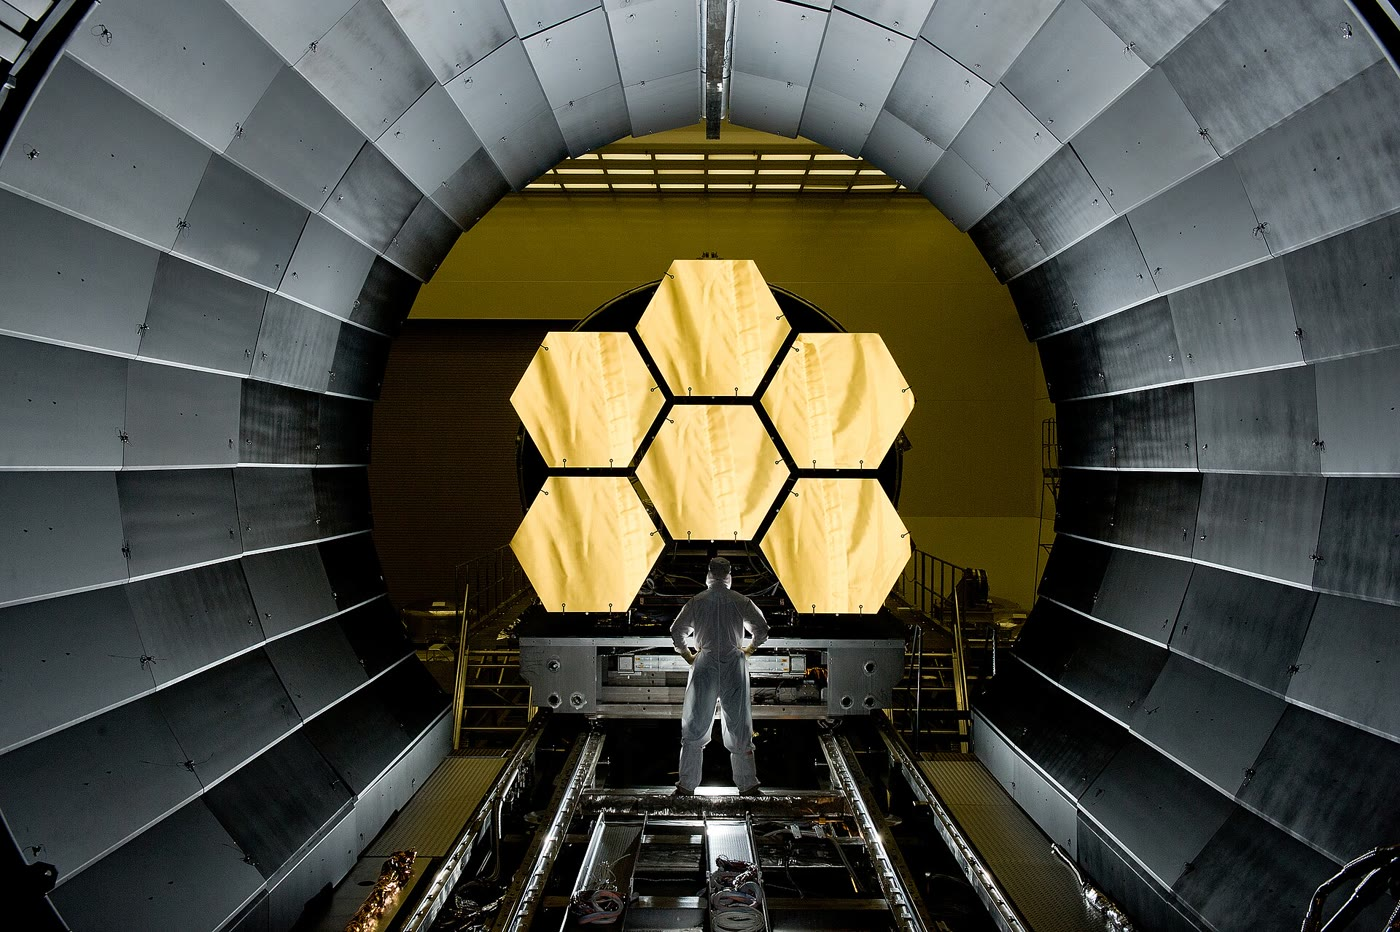
\includegraphics[width=0.78\linewidth]{images/book3/b1-jwst-mirror-segments.jpg}

{\small Six of the 18 hexagonal segments of the James Webb Space Telescope's
primary mirror, prepared for cold testing in 2011; together, unfolded in
space, the 18 form a mirror \qty{6.5}{m} wide. Photograph NASA/MSFC/David Higginbotham,
public domain.}
% ledger: commons:jwst-mirror, nasa:jwst-mirror
\end{omfigure}

\section{Exercises}

\begin{exercise}[$\star$]\label{exo:b1:observing-the-sky:1}
What is the ratio of the \omterm{def:b1:observing-the-sky:flux}{fluxes} of two stars of magnitudes 1.0 and 6.0? Of
Rigel ($V = 0.13$) and Polaris ($V = 2.02$)? Which is brighter in the sky?
\end{exercise}

\begin{exercise}[$\star$]\label{exo:b1:observing-the-sky:2}
The parallax of Altair is \ang{;;0.19495}. Give its distance in \omterm{def:b1:observing-the-sky:parallax}{parsecs}, in
astronomical units and in light-years.
\end{exercise}

\begin{exercise}[$\star$]\label{exo:b1:observing-the-sky:3}
Compute the diffraction limit of a \qty{2.4}{m} space telescope at
\qty{550}{nm}, in seconds of arc, and compare it with a \omterm{def:b1:observing-the-sky:seeing}{seeing} of
\ang{;;0.40}. Do the same for a \qty{6.5}{m} telescope at
\qty{2.0}{\micro\metre}.
\end{exercise}

\begin{exercise}[$\star$]\label{exo:b1:observing-the-sky:4}
From the table of the four bright stars, rank Rigel, Altair, Polaris and
Betelgeuse from the hottest surface to the coolest. Why can the \omterm{def:b1:observing-the-sky:colour-index}{colour index}
be compared between stars at very different distances?
\end{exercise}

\begin{exercise}[$\star\star$]\label{exo:b1:observing-the-sky:5}
A star is measured at the magnitude 6.412 at the \omterm{def:b1:spherical-astronomy:celestial-sphere}{zenith} distance \ang{30}
and at 6.590 at \ang{60} on the same night. Assuming a plane-parallel
atmosphere, compute the two airmasses, the extinction coefficient and the
magnitude of the star above the atmosphere.
\end{exercise}

\begin{exercise}[$\star\star$]\label{exo:b1:observing-the-sky:6}
A star gives 400 photoelectrons in a \qty{10}{s} exposure, and photon noise
from the star alone dominates. What is the \omterm{def:b1:observing-the-sky:detector}{signal-to-noise ratio}? How long
must one expose to reach an SNR of 100? To measure the magnitude to
\num{0.01}?
\end{exercise}

\begin{exercise}[$\star\star$]\label{exo:b1:observing-the-sky:7}
Rigel has $V = 0.13$ and a parallax of \ang{;;0.00378}. Neglecting
extinction between it and us, compute its distance, its \omterm{def:b1:observing-the-sky:absolute}{absolute magnitude}
and its V-band \omterm{def:b1:observing-the-sky:flux}{luminosity} in solar units ($M_\odot = 4.83$).
\end{exercise}

\begin{exercise}[$\star\star$]\label{exo:b1:observing-the-sky:8}
Compare the collecting areas of a \qty{2.4}{m} circular mirror (ignore its
central obstruction) and of the Webb telescope (\qty{25}{m^2}). How much
shorter is the exposure in which the Webb telescope collects the same number
of photons? What fraction of a full disc \qty{6.5}{m} across does its
collecting area represent, and why is it less than one?
\end{exercise}

\begin{exercise}[$\star\star$]\label{exo:b1:observing-the-sky:9}
(a) From the Sun's \omterm{def:b1:observing-the-sky:flux}{luminosity}, \qty{3.828e26}{W}, compute its \omterm{def:b1:observing-the-sky:flux}{flux} at
\qty{10}{\parsec}. (b) The Sun's apparent and \omterm{def:b1:observing-the-sky:absolute}{absolute magnitudes} are
$-26.74$ and $4.83$. Use the \omterm{def:b1:observing-the-sky:absolute}{distance modulus} to recover the Sun--Earth
distance, in astronomical units.
\end{exercise}

\begin{exercise}[$\star\star\star$]\label{exo:b1:observing-the-sky:10}
Show from \cref{prop:b1:observing-the-sky:bouguer} that $k =
2.5\log_{10}e\;\tau_0$. For the night of the extinction line ($k =
\num{0.160}$), compute the \omterm{def:b1:spherical-astronomy:celestial-sphere}{zenith} optical depth $\tau_0$ and the fraction of
the light that reaches the telescope at the \omterm{def:b1:spherical-astronomy:celestial-sphere}{zenith} and at $X = 2.31$. What
would a plane-parallel atmosphere predict for the \omterm{def:b1:observing-the-sky:extinction}{airmass} at a \omterm{def:b1:spherical-astronomy:celestial-sphere}{zenith}
distance of \ang{85}, and why should that value not be trusted?
\end{exercise}

\begin{exercise}[$\star\star\star$]\label{exo:b1:observing-the-sky:11}
A faint galaxy gives $R = 50$ photoelectrons per second in a telescope, and
the sky in the area of its image gives $B = \num{2000}$ per second when the
\omterm{def:b1:observing-the-sky:seeing}{seeing} is \ang{;;0.80}. Read noise is negligible. (a) How long must one
expose for an SNR of 10? (b) The sky in the image grows as the area of the
\omterm{def:b1:observing-the-sky:seeing}{seeing} disc. Repeat for a \omterm{def:b1:observing-the-sky:seeing}{seeing} of \ang{;;0.40}. (c) Show that, for a
source much fainter than the sky, the exposure time needed for a given SNR
varies as $\theta^2/D^2$, where $\theta$ is the \omterm{def:b1:observing-the-sky:seeing}{seeing} and $D$ the diameter
of the telescope.
\end{exercise}

\begin{exercise}[$\star\star\star$]\label{exo:b1:observing-the-sky:12}
A grating with 1200 lines per millimetre is illuminated over \qty{100}{mm}
and used in the first order. (a) What is its resolving power, and the
smallest separable wavelength difference at \qty{550}{nm}? (b) What radial
velocity does that difference correspond to? (c) The Earth moves round the
Sun at \qty{29.78}{km.s^{-1}}. By how much can that motion shift a line at
\qty{550}{nm}, and how many resolution elements is that? What must an
observer measuring a star's velocity therefore do?
% ledger: earth:vorb
\end{exercise}

\section{Problem: Weighing the light of Sirius}

\begin{problem}[{Weekend problem --- how far Sirius is, how bright it looks
and how many photons it sends, and how many suns it outshines}]
\label{pb:b1:observing-the-sky:1}
% ledger: simbad:sirius, simbad:vega, simbad:sirius-b, nasa:sun-V, sun:Mabs, const:au
% numbers computed in the scratch calculator calc/ch02.py from the rounded data
Sirius, the brightest star of the night sky, has a faint companion, the
white dwarf Sirius~B. Use the data:
\begin{center}
\small
\begin{tabular}{lcc}
\hline
object & $V$ & parallax \\
\hline
Sirius & $-1.46$ & \ang{;;0.37921} \\
Sirius B & $8.44$ & --- \\
Vega & $0.03$ & \ang{;;0.13023} \\
the Sun & $-26.74$ & --- \\
\hline
\end{tabular}
\end{center}
with $M_\odot = 4.83$ in V, $\qty{1}{\parsec} = \qty{206265}{\au} =
\qty{3.0857e16}{m} = \qty{3.2616}{\lightyear}$, and an extinction
coefficient $k = 0.15$ per \omterm{def:b1:observing-the-sky:extinction}{airmass} at the observatory.

\medskip
\noindent\textbf{Part I --- How far is Sirius?}
\begin{enumerate}
  \item Compute the distance of Sirius in \omterm{def:b1:observing-the-sky:parallax}{parsecs}.
  \item Express it in astronomical units and in metres.
  \item Express it in light-years. How long ago did the light we see
        tonight leave Sirius?
  \item Over a year, by what total angle does the direction of Sirius
        swing from side to side? Compare it with a \omterm{def:b1:observing-the-sky:seeing}{seeing} of \ang{;;0.40}.
        Why can the swing still be measured to a small fraction of the
        \omterm{def:b1:observing-the-sky:seeing}{seeing}?
  \item If the parallax were wrong by \ang{;;0.001}, by what fraction would
        the distance be wrong, and by how many light-years?
\end{enumerate}

\medskip
\noindent\textbf{Part II --- How bright does it look?}
\begin{enumerate}[resume]
  \item Compute the ratio of the \omterm{def:b1:observing-the-sky:flux}{fluxes} of Sirius and Vega in V.
  \item Compute the ratio of the \omterm{def:b1:observing-the-sky:flux}{fluxes} of the Sun and Sirius.
  \item Compute the ratio of the \omterm{def:b1:observing-the-sky:flux}{fluxes} of Sirius and of Sirius~B.
  \item From the Paranal Observatory, Sirius crosses the meridian at an
        \omterm{def:b1:spherical-astronomy:horizontal}{altitude} of \ang{82.09} (\cref{ch:b1:spherical-astronomy}). Compute
        the \omterm{def:b1:observing-the-sky:extinction}{airmass}, the extinction, and the magnitude measured at that
        moment.
  \item Repeat at an \omterm{def:b1:spherical-astronomy:horizontal}{altitude} of \ang{30}. What fraction of the light is lost
        on the way?
  \item Why would the formula $X = \sec z$ mislead an observer measuring
        Sirius just after it rises?
\end{enumerate}

\medskip
\noindent\textbf{Part III --- Counting photons.}
A camera on a \qty{1}{m} telescope records $\num{3.0e4}$ photoelectrons per
second from a star of magnitude $V = 10.0$, once corrected for extinction.
Each pixel holds at most $\num{1.0e5}$ electrons (its full well).
\begin{enumerate}[resume]
  \item How many photoelectrons per second does the camera record from
        Sirius~B?
  \item How long an exposure gives Sirius~B an SNR of 1000, with photon
        noise from the star alone? What is then the error on its magnitude?
  \item How many photoelectrons per second does the camera record from
        Sirius?
  \item If \qty{20}{\percent} of the light of Sirius falls in its brightest
        pixel, how long does that pixel take to fill?
  \item On the image, the faint wings of Sirius's image deposit, at the
        place of Sirius~B, $10^{-4}$ of the light of Sirius per pixel, and
        Sirius~B's brightest pixel collects \qty{20}{\percent} of its own
        light. Compare the two rates in that pixel.
  \item What is the longest exposure that does not saturate that pixel?
        Compute the SNR of Sirius~B in that pixel in an exposure of
        \qty{0.5}{s}, counting the photon noise of both sources. Is Sirius~B
        detectable, and what makes it hard?
\end{enumerate}

\medskip
\noindent\textbf{Part IV --- How many suns?}
\begin{enumerate}[resume]
  \item Compute the \omterm{def:b1:observing-the-sky:absolute}{distance modulus} of Sirius.
  \item Deduce the \omterm{def:b1:observing-the-sky:absolute}{absolute magnitude} of Sirius in V, to two decimals.
  \item Compute the distance and the \omterm{def:b1:observing-the-sky:absolute}{absolute magnitude} of Vega.
  \item Which of Sirius and Vega is intrinsically more luminous in V, and
        by what factor?
  \item What would be the \omterm{def:b1:observing-the-sky:magnitude}{apparent magnitude} of the Sun seen from the
        distance of Sirius? Taking 6.0 as the faintest magnitude visible to
        the naked eye on a dark night, would it be visible?
  \item Out to what distance would Sirius remain visible to the naked eye?
  \item Compute the V-band \omterm{def:b1:observing-the-sky:flux}{luminosity} of Sirius in solar units: how many
        suns does Sirius outshine?
\end{enumerate}
\end{problem}
